%!TEX root = ../../Master.tex
\section{Storing A Graph}

This chapter will discuss different methods of storing a graph in memory for a C program to interpret and compute. Furthermore how to read a model of a hospital from a XML document.

\subsection{Sequentially Representation}
A Sequential representation means that the data describing the vertices is placed sequentially in the memory, one vertex after another. The overhead of storing the memory sequentially is very small. Appending a new element to the list is very easy, because the exact location in memory is known. However when inserting an element in the middle of a sequentially list, up to half of the elements need to be moved by 1 position. 



% It can be done by changing what the last element of the list is pointing at, to a new element.
% Removing an item can be done similarly by changing the element pointing to the item that is wanted to be removed, so the list skips a element. This is shown in \cref{fig:examplegraph}.


\subsection{Linked List Representation}
\label{sub:list}
A linked list is defined as \enquote{a list implemented by each item having a link to the next item} \cite{linked_list_def}. This means that every item in the list has a element pointing to the next item in the list. This way of structuring the data makes it possible to dynamic manipulate the list \cite{Linked_List}.  Doing this means that the overhead of storing a linked list is a little bigger than storing a list sequential, because of the next pointers also consume memory. 

Inserting new items to a linked list is relatively easy, compared to sequentially storing memory. This can be done by redirecting a pointer to an element $A$ in the list to a newly created element $B$, and make the the new element point at location where the first element was pointing to $C$. This example is shown at \cref{fig:link}.

\begin{figure}[h]
 \centering
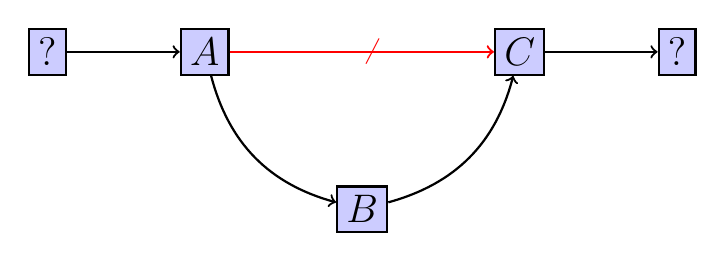
\begin{tikzpicture}[thick,main node/.style={fill=blue!20,draw,font=\sffamily\Large\bfseries}]
  \node[main node] (a) at (0,0) {\(A\)};
  \node[main node] (c) at (4,0) {\(C\)};
  \node[main node] (b) at (2,-2) {\(B\)};
  \node[main node] (d) at (-2,0) {$?$};
  \node[main node] (e) at (6,0) {$?$};
   
   \path[->]
     (d) edge node {$ $} (a)
     (c) edge node {$ $} (e)
     (a) edge [bend right] node {$ $} (b)
     (b) edge [bend right] node {$ $} (c);

  \draw[red,->] (a) to node {\(\not\)} (c);
\end{tikzpicture}
\caption{Linked list example} \label{fig:link}
\end{figure}
 %indsæt 


% \subsection{data structure}
% In this section it will be covered how a graph actual can be represented in the memory, using the above methods. To explain this there examples in the following sections will be based on the graph shown at \cref{fig:graph}.
% \begin{figure}[h]
% \centering
% \begin{tikzpicture}[->,>=stealth',shorten >=1pt,auto,node distance=3cm,
%   thick,main node/.style={circle,fill=blue!20,draw,font=\sffamily\Large\bfseries}]

%   \node[main node] (1) {1};
%   \node[main node] (2) [below left of=1] {2};
%   \node[main node] (3) [below right of=1] {3};
%   \path[-]
%   	(1) edge node {2.0} (3)
%     (2) edge node {1.0} (1)
%     (3) edge node {3.0} (2);
% \end{tikzpicture}
% \caption{example graph} \label{fig:graph}
% \end{figure}




% \begin{figure}[h]
% \centering
% \begin{tikzpicture}[->,>=stealth',shorten >=1pt,auto,node distance=3cm,thick,main node/.style={fill=blue!20,draw,font=\sffamily\Large\bfseries}]

%   \tikzset{mystyle/.style={->,relative=false,in=0,out=0,bend left=100,looseness=3}}

%   \node[main node] at (0,-2) (2) {$V_1$};
%   \node[main node] at (2,-2) (3) {$V_2$};
%   \node[main node] at (4,-2) (4) {$V_3$};
%   \node[main node] at (0,-4) (5) {$EP_1$};
%   \node[main node] at (2,-4) (7) {$EP_2$};
%   \node[main node] at (4,-4) (9) {$EP_1$};
%   \node[main node,label=below:$1$] at (0,-6) (6) {$E_1$};
%   \node[main node,label=below:$1$] at (2,-6) (8) {$E_1$};

%    \path[->]
%    	(2) edge node {VP} (3)
%    	(3) edge node {VP} (4)
%    	(2) edge node {EP} (5)
%    	(5) edge node {EP} (6)
%    	(5) edge node {EP} (7)
%    	(7) edge node {EP} (8)
%    	(6) edge [bend left=60] node { } (2)
%    	(6) edge [bend left=100,looseness=2.3] node { }(3)
%    	(8) edge [bend left=100,looseness=2.5] node { }(2)
%    	(8) edge [bend right=100,label=right] node { }(4);


% \end{tikzpicture}
% \caption{example graph} \label{fig:examplegraph}
% \end{figure}

\subsection{Representing a Graph as XML}

In order to search through a graph in a C program, the graph needs to be read by the C program. XML was chosen as the markup language for representing a graph, because of its readability for both humans and computers. An example of how a graph is represented as XML is seen in \cref{list:xml_demo}.

\lstinputlisting[language=XML, label=list:xml_demo, caption={An example of a graph represented as XML}]{Chapters/problem_solution/demo_xml.xml}

%!TEX root = ../../Master.tex

\subsection{Data Structure}
\label{sub:data_structure}

This subsection will cover which way of representing a graph that has been chosen. The solution was to break the graph in to small pieces of information, this made it easier to keep track of the program. It was chosen to split the datasets in to 5 structs.
\begin{minipage}{\linewidth}
\begin{itemize} [noitemsep]
	\item Graph
	\item Floor
	\item Vertex
	\item Edge Pointer
	\item Edge
\end{itemize}
\end{minipage}

These structs will be explained in the following sections. 

%In \cref{Implementing}, the advantages and disadvantages of a linked list and a array was described.
\begin{minipage}{\linewidth}
\subsection{Graph} 
This is the main struct containing information of one building complex.
The struct have a pointer called floors that points to the first floor struct that contains information about one floor. All floors is sequentially stored in the memory so by incrementing the pointer it is possible to access the next element. How we represent another building is described in \cref{multlayhan}. The element numOfVertices contains how many vertecies this graph have in total, and numOfFloors is how many floors this graph have.


\lstinputlisting[language=C, frame=single, numbers=left]{Chapters/problem_solution/graph.c} \label{Graph_struct}
\end{minipage}

\begin{minipage}{\linewidth}
\subsection{Floor} \label{subsub:floor}
This struct reasonably simple the functionality of it, is to separate vertecies so a floor only contains a vertecies that is located a the same floor. The $floorId$ is an identifier to keep track of which floor that are in use.
$amountOfVertecies$ is a values telling how many vertecies this floor have. Vp is a pointer to the first vertex in this floor.

\lstinputlisting[language=C, frame=single, numbers=left]{Chapters/problem_solution/Floor.c} \label{Floor_struct}
\end{minipage}

\begin{minipage}{\linewidth}
\subsection{Vertex}\label{data_struct:vertex}
A vertex struct holds information about where it is located relative to other vertecies using a cordinat set $x$ and $y$. Vertecies can be identified using the $vertexId$, the $floorId$ is used to tell whether to vertecies is at the same layer.

 The $type$ can represent:
\begin{itemize}[noitemsep]
	\item \textbf{1}: Normal vertex.
	\item \textbf{2}: Stair vertex.
	\item \textbf{3}: Elevator vertex.
\end{itemize}

The $ep$ is a pointer to the first element in a linked list row, each element is contains a pointer to the next $Edge pointer$ that this vertex is connected to. The benefits of this representations method is described in \cref{sub:list} and makes it possible to add edges to this vertex after initialization.


All vertecies on in the same floor is connected using a linked list. This makes it possible to dynamic add new vertecies to the floor as described in \cref{sub:list}. The start of the list is pointed to by the floor struct. It is important to mention that the order of the list plays no role.   


\lstinputlisting[language=C, frame=single, numbers=left]{Chapters/problem_solution/vertex.c} \label{vertex_struct}
\end{minipage}

\begin{minipage}{\linewidth}
\subsection{Edge Pointer}
The edge pointer struct have two elements one pointing to the $edge$ containing information about the cost of the edge and which vetecies it is connected to. And the other element $nextEp$ points to the next edge pointer this Vertex is connected to. When a $nextEp$ is pointing to $NULL$ the end of the list is reached.
\lstinputlisting[language=C, frame=single, numbers=left]{Chapters/problem_solution/ep.c} \label{ep_struct}
\end{minipage}



\begin{minipage}{\linewidth}
\subsection{Edge}
The last struct is the $edge$ struct, this struct is pointed to by two vertecies using a $edge$ pointer. The same to vertecies is pointed to by the $edge$, using the two $Vertex$ pointers. This represent with vertices is connected.
The $edgeId$ used while parsing XML code, to keep track of which vertex is connected to which vertex.
This is is done because a pointer to an edge cant be stored in files, so ids is used to represent a pointer. 
\lstinputlisting[language=C, frame=single, numbers=left]{Chapters/problem_solution/edge.c} \label{edge_struct}
\end{minipage}


\subsection{Summary of Graph Theory}

The sequentially representation requires less memory, and adding or removing elements is also easier compared to a linked list representation, which have meant that the sequentially representation  have been chosen for representing a graph 


\begin{figure}[h]
\centering
\begin{tikzpicture}[->,>=stealth',shorten >=1pt,auto,node distance=3cm,thick,main node/.style={fill=blue!20,draw,font=\sffamily\Large\bfseries}]

  \tikzset{mystyle/.style={->,relative=false,in=0,out=0,bend left=100,looseness=3}}

  \node[main node] at (0,-2) (2) {$V_1$};
  \node[main node] at (2,-2) (3) {$V_2$};
  \node[main node] at (4,-2) (4) {$V_3$};
  \node[main node] at (0,-4) (5) {$EP_1$};
  \node[main node] at (2,-4) (7) {$EP_2$};
  \node[main node,label=below:$1$] at (0,-6) (6) {$E_1$};
  \node[main node,label=below:$1$] at (2,-6) (8) {$E_2$};

   \path[->]
   	(2) edge node {VP} (3)
   	(3) edge node {VP} (4)
   	(2) edge node {EP} (5)
   	(5) edge node {EP} (6)
   	(5) edge node {EP} (7)
   	(7) edge node {EP} (8)
   	(6) edge [bend left=60] node { } (2)
   	(6) edge [bend left=100,looseness=2.3] node { }(3)
   	(8) edge [bend right=30,label=right] node { }(4)
   	(8) edge [bend right=100,looseness=3] node { }(2);


\end{tikzpicture}
\caption{example graph} \label{fig:examplegraph}
\end{figure}


